\chapter{Image restoration}

\section{Problem statement}

Suppose a blurring degradation function as
\begin{equation}
    H(u, v) = T \times sinc(ua + vb) \times e^{-j\pi(ua + vb)}
\end{equation}
\bigskip
\begin{enumerate}[(a)]
    \item Implement a blurring filter using the equation above.
    \item Blur the test image book\_cover.jpg using parameters $a = b = 0.1$ and $T = 1$.
    \item Add Gaussian noise of $0$ mean and variance of $650$ to the blurred image.
    \item Restore the blurred image and the blurred noisy image using the inverse filter,
          Wiener deconvolution filter and the parametric Wiener filter, respectively.
      \item Add Gaussian noise of $0$ and different variances to the blurred image and repeat (d),
          investigate the performance of the Wiener deconvolution filter.
\end{enumerate}

\section{Python implementation}

Usage:~\textbf{problem5.py [-h] [--blurred BLURRED] [--noise] [-s S] [--inv]} \\
\textbf{[--wiener] [-a A] [-b B] [-T T] [-K K]}
\textbf{image\_path} \\\\
Use \textbf{python problem5.py -h} to see the help.

\pagebreak
\section{Blurring and noising}

\textbf{python problem5.py book\_cover.jpg}

\begin{figure}[!htb]\centering
    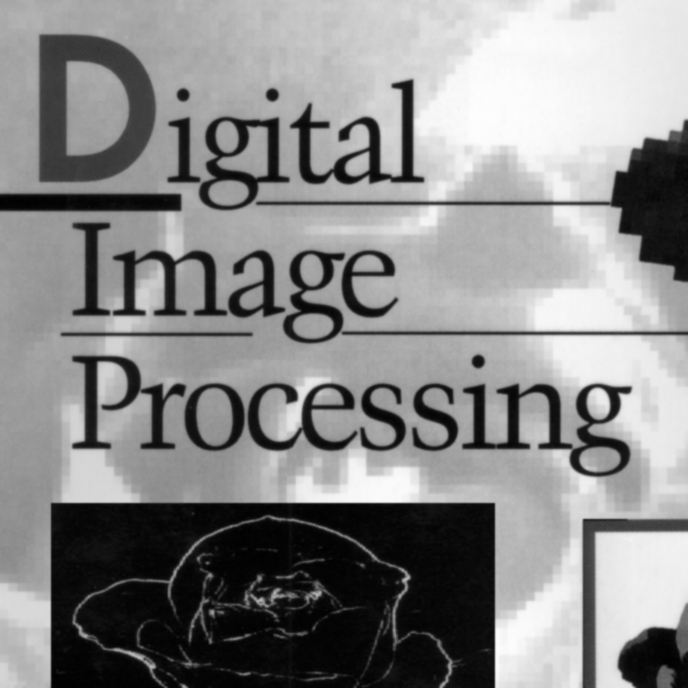
\includegraphics[width=0.6\linewidth]{./images/5/original.jpg}
    \caption{\small{Original image}}
\end{figure}

\begin{figure}[!htb]\centering
    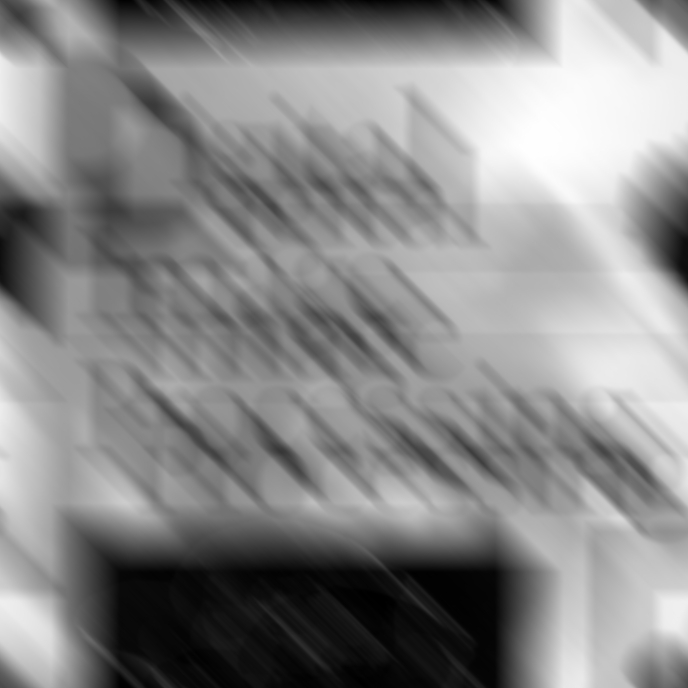
\includegraphics[width=0.6\linewidth]{./images/5/blurred.jpg}
    \caption{\small{Blurred image ($a = b = 0.1; T = 1$)}}\label{diagram:blurred}
\end{figure}


\pagebreak
\textbf{python problem5.py book\_cover.jpg --noise -s 650}

\begin{figure}[!htb]\centering
    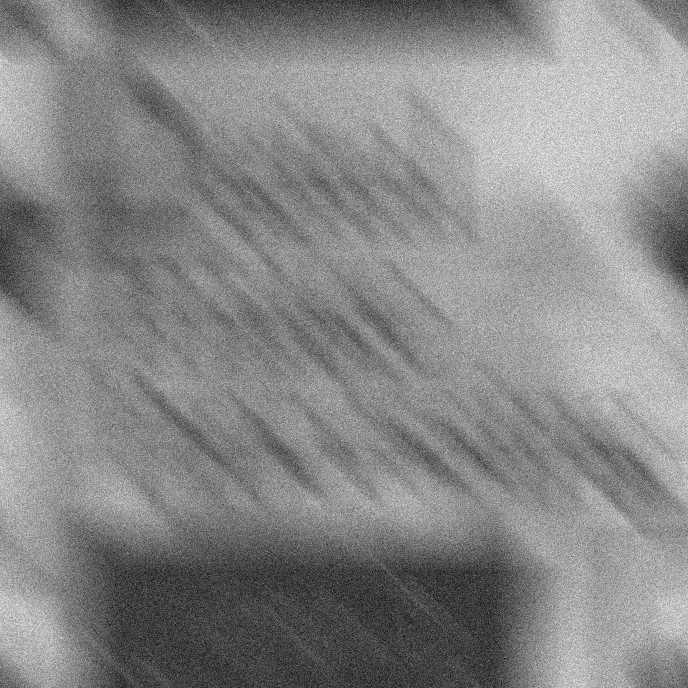
\includegraphics[width=0.6\linewidth]{./images/5/blurred_noise.jpg}
    \caption{\small{Blur + Gaussian noise ($\mu = 0, \sigma^2 = 650$)}}\label{diagram:blurred_noise}
\end{figure}


\pagebreak
\section{Restoration}

\subsection{Inverse filter}

\begin{minipage}{\textwidth}
\textbf{python problem5.py --inv book\_cover.jpg} \\
\textbf{python problem5.py --noise -s 650 --inv book\_cover.jpg}
\end{minipage}

\begin{figure}[!htb]\centering
    \begin{minipage}{0.45\textwidth}
        \frame{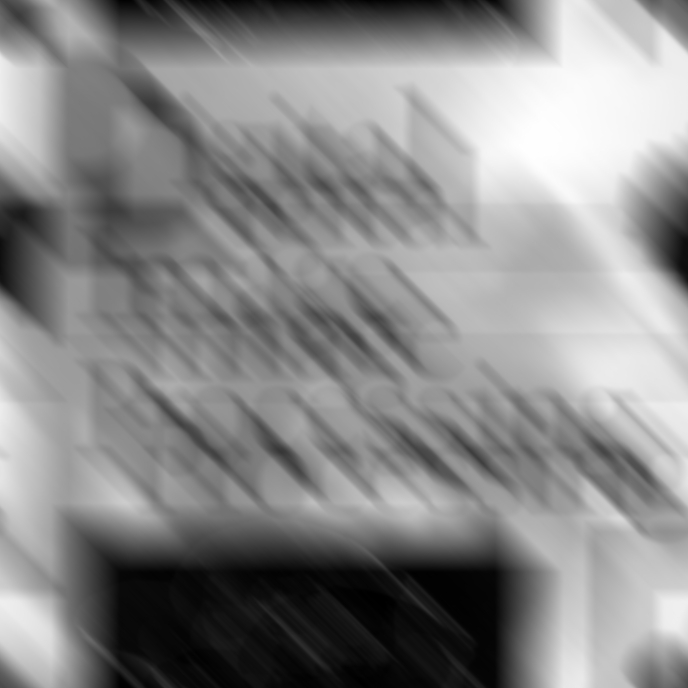
\includegraphics[width=\linewidth]{./images/5/blurred.jpg}}
        \caption{\small{Blurred image}}
    \end{minipage}
    \begin{minipage}{0.45\textwidth}
        \frame{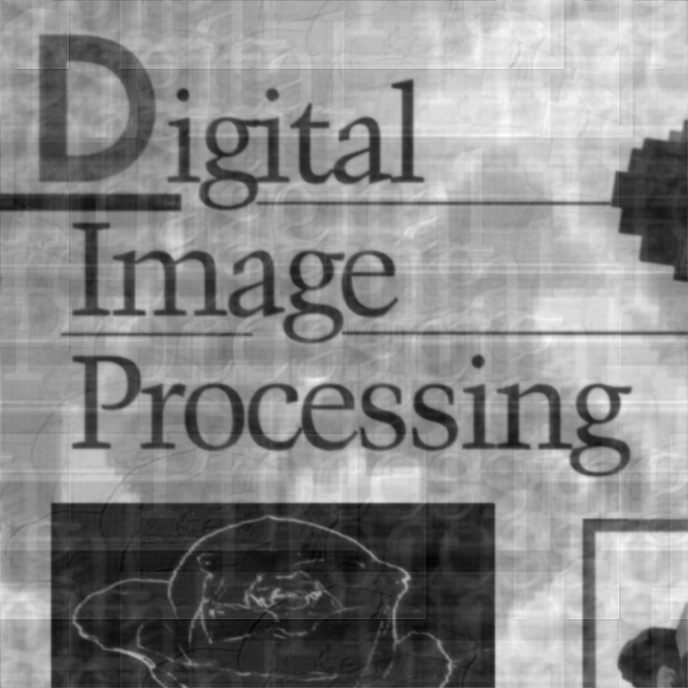
\includegraphics[width=\linewidth]{./images/5/inv_blurred.jpg}}
        \caption{\small{Inverse blurred image}}\label{diagram:inv_blurred}
    \end{minipage}
\end{figure}

\begin{figure}[!htb]\centering
    \begin{minipage}{0.45\textwidth}
        \frame{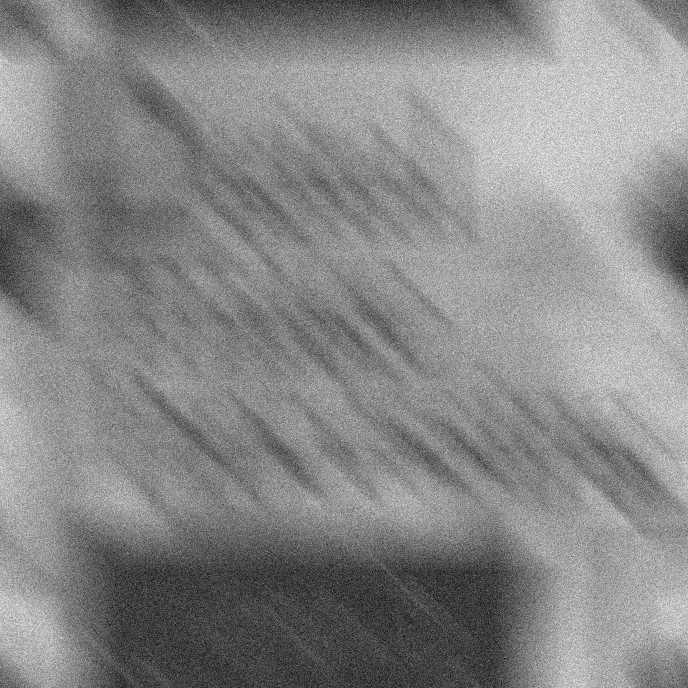
\includegraphics[width=\linewidth]{./images/5/blurred_noise.jpg}}
        \caption{\small{Blur + noise}}
    \end{minipage}
    \begin{minipage}{0.45\textwidth}
    \frame{
\includegraphics[width=\linewidth]{./images/5/inv_blurred_noise.jpg}}
    \caption{\small{Inverse 'blur + noise'}}\label{diagram:inv_blurred_noise}
    \end{minipage}
\end{figure}
\bigskip
The inverse filter is really affected by the noise because it ignores it (does not inverse it).

\pagebreak
\subsection{Wiener filter}
\begin{minipage}{\textwidth}
\textbf{python problem5.py --wiener book\_cover.jpg} \\
\textbf{python problem5.py --noise -s 650 --wiener book\_cover.jpg}
\end{minipage}

\begin{figure}[!htb]\centering
    \begin{minipage}{0.45\textwidth}
        \frame{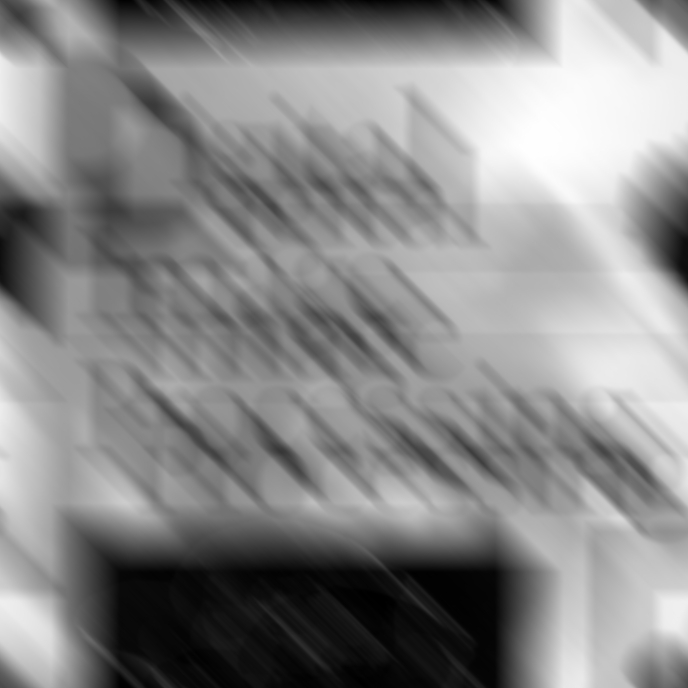
\includegraphics[width=\linewidth]{./images/5/blurred.jpg}}
        \caption{\small{Blurred image}}
    \end{minipage}
    \begin{minipage}{0.45\textwidth}
        \frame{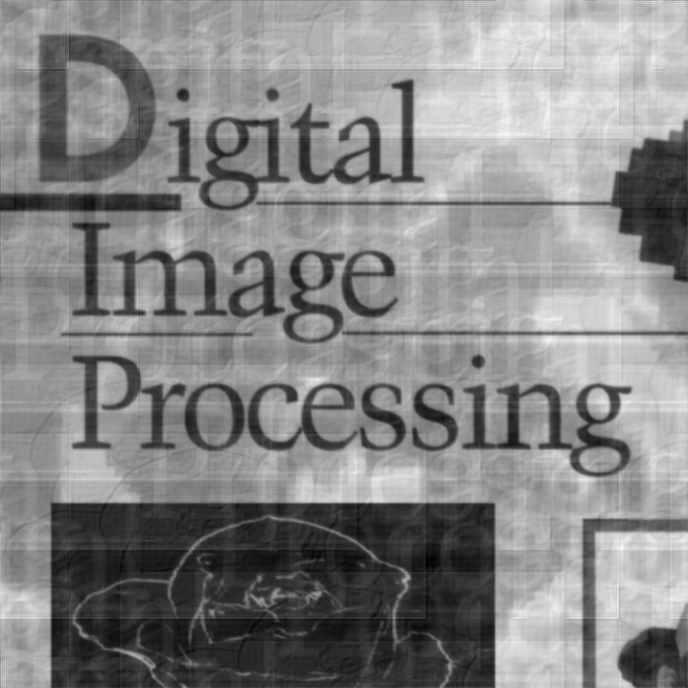
\includegraphics[width=\linewidth]{./images/5/wiener_blurred.jpg}}
        \caption{\small{Wiener blurred image}}\label{diagram:wiener_blurred}
    \end{minipage}
\end{figure}

\begin{figure}[!htb]\centering
    \begin{minipage}{0.45\textwidth}
        \frame{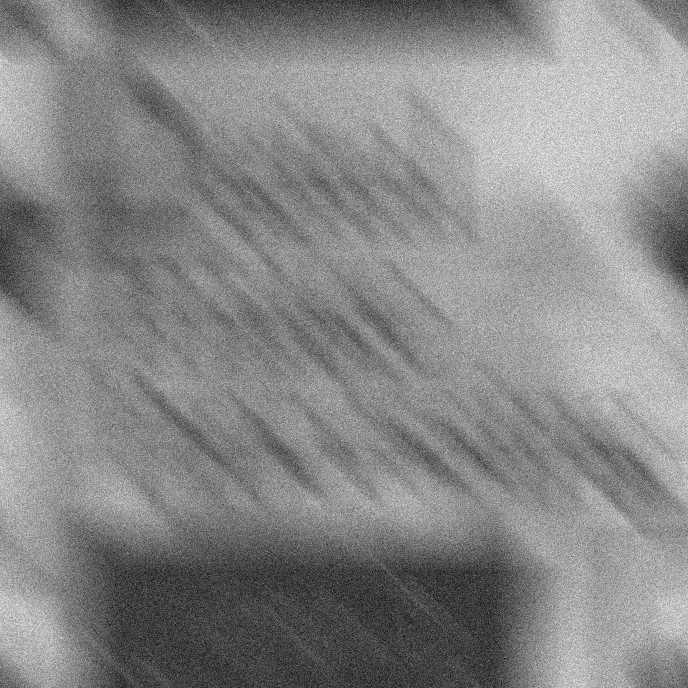
\includegraphics[width=\linewidth]{./images/5/blurred_noise.jpg}}
        \caption{\small{Blur + noise}}
    \end{minipage}
    \begin{minipage}{0.45\textwidth}
    \frame{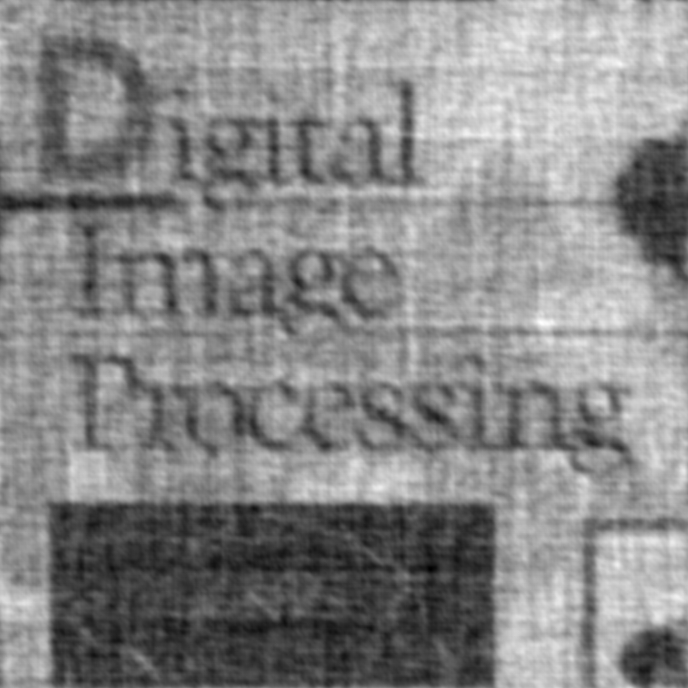
\includegraphics[width=\linewidth]{./images/5/wiener_blurred_noise.jpg}}
    \caption{\small{Wiener 'blur + noise'}}\label{diagram:wiener_blurred_noise}
    \end{minipage}
\end{figure}
\bigskip
The Wiener filter on the blurred image without noise is equivalent to the inverse filter (power spectrum of noise equals to 0). \\
The Wiener filter is more efficient to remove the noise as it takes it into consideration
during the restoration process.

\pagebreak
\subsection{Parametric Wiener filter}
TODO

\pagebreak
\subsection{Experimentations}

\subsubsection{Gaussian noise ($\mu = 0, \sigma^2 = 300$)}

\begin{figure}[!htb]\centering
    \begin{minipage}{0.45\textwidth}
        \frame{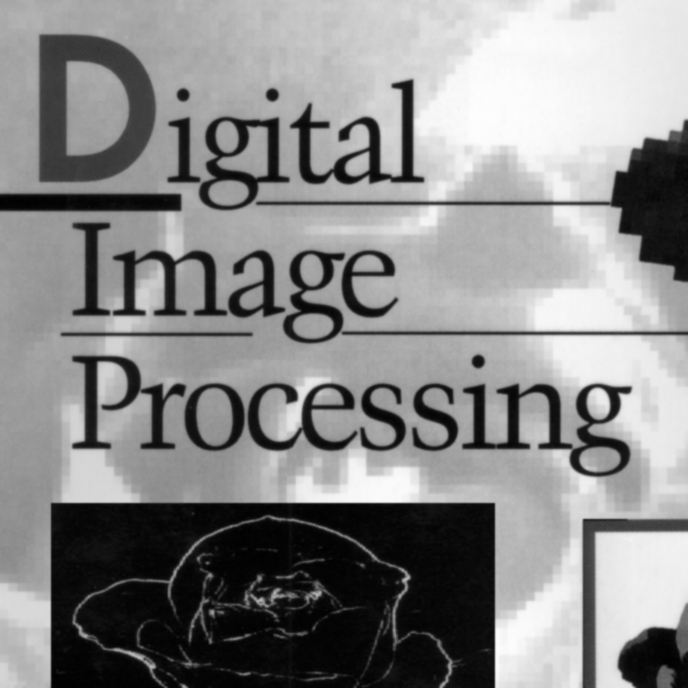
\includegraphics[width=\linewidth]{./images/5/original.jpg}}
        \caption{\small{Original image}}
    \end{minipage}
    \begin{minipage}{0.45\textwidth}
        \frame{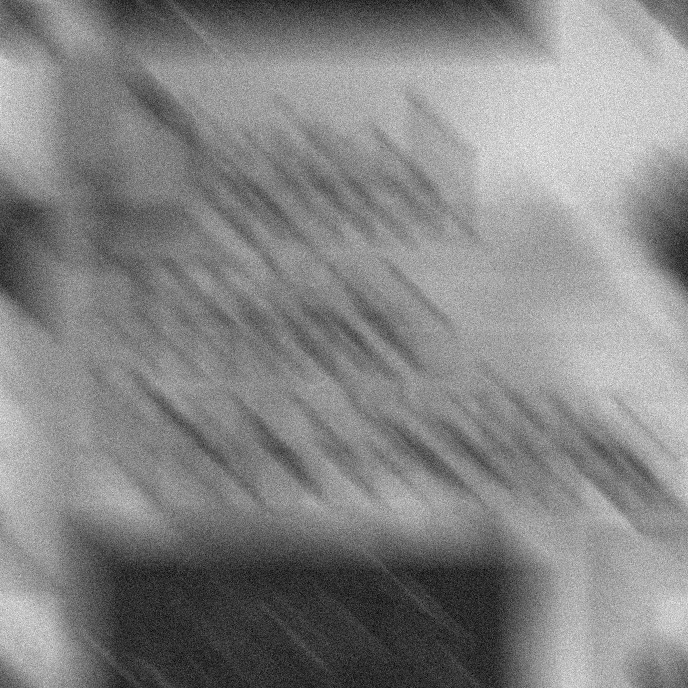
\includegraphics[width=\linewidth]{./images/5/blurred_noise_300.jpg}}
        \caption{\small{Blur + noise}}
    \end{minipage}
\end{figure}

\begin{figure}[!htb]\centering
    \begin{minipage}{0.45\textwidth}
        \frame{
\includegraphics[width=\linewidth]{./images/5/inv_blurred_noise_300.jpg}}
        \caption{\small{Inverse 'blur + noise'}}
    \end{minipage}
    \begin{minipage}{0.45\textwidth}
    \frame{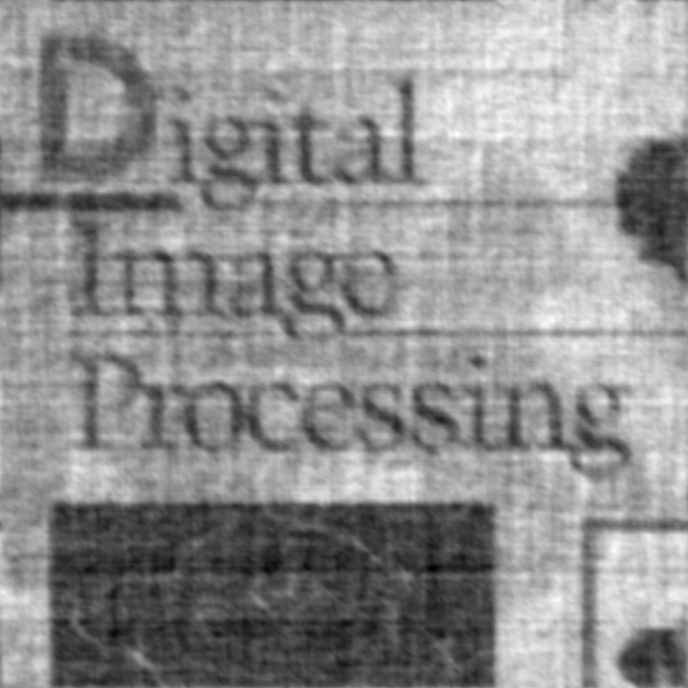
\includegraphics[width=\linewidth]{./images/5/wiener_blurred_noise_300.jpg}}
    \caption{\small{Wiener 'blur + noise'}}
    \end{minipage}
\end{figure}

\pagebreak
\subsubsection{Gaussian noise ($\mu = 0, \sigma^2 = 100$)}

\begin{figure}[!htb]\centering
    \begin{minipage}{0.45\textwidth}
        \frame{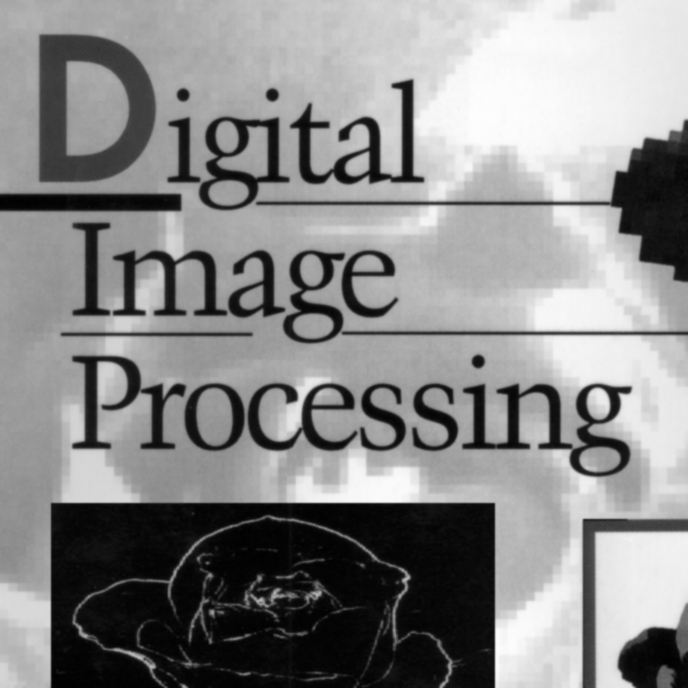
\includegraphics[width=\linewidth]{./images/5/original.jpg}}
        \caption{\small{Original image}}
    \end{minipage}
    \begin{minipage}{0.45\textwidth}
        \frame{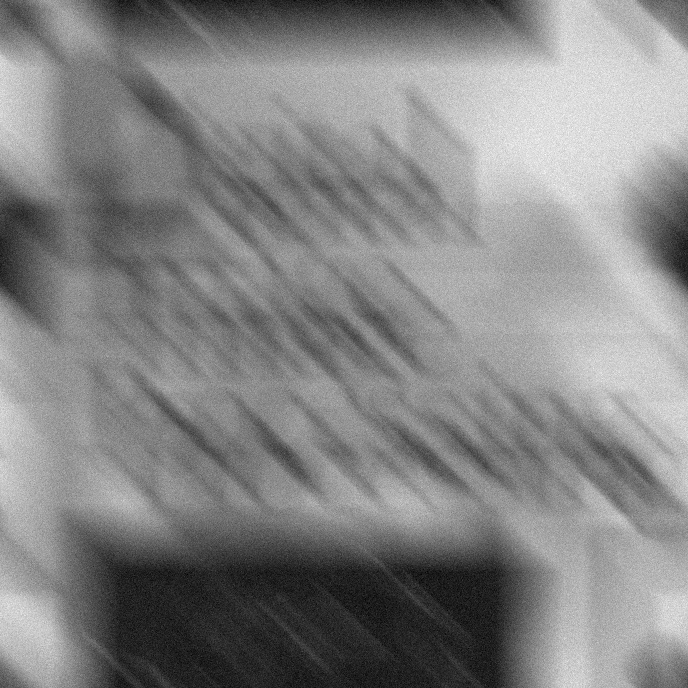
\includegraphics[width=\linewidth]{./images/5/blurred_noise_100.jpg}}
        \caption{\small{Blur + noise}}
    \end{minipage}
\end{figure}

\begin{figure}[!htb]\centering
    \begin{minipage}{0.45\textwidth}
        \frame{
\includegraphics[width=\linewidth]{./images/5/inv_blurred_noise_100.jpg}}
        \caption{\small{Inverse 'blur + noise'}}
    \end{minipage}
    \begin{minipage}{0.45\textwidth}
    \frame{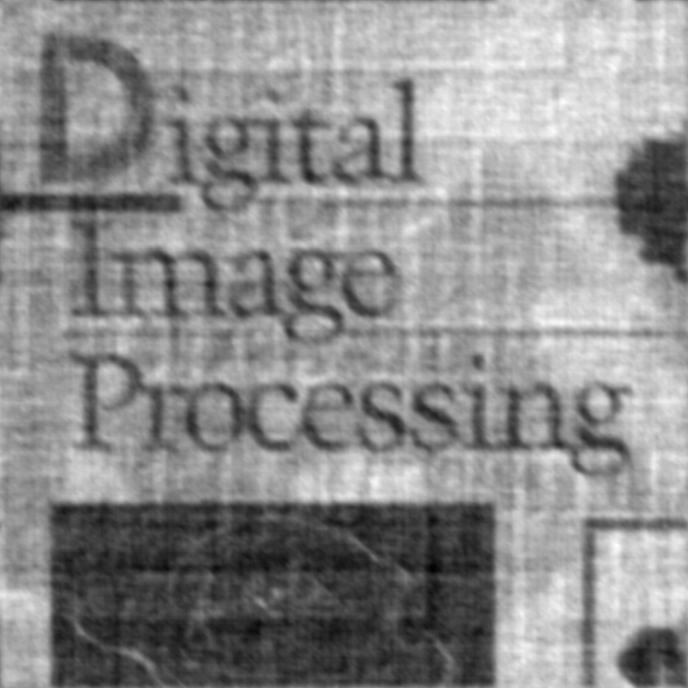
\includegraphics[width=\linewidth]{./images/5/wiener_blurred_noise_100.jpg}}
    \caption{\small{Wiener 'blur + noise'}}
    \end{minipage}
\end{figure}

\pagebreak
\subsubsection{Gaussian noise ($\mu = 0, \sigma^2 = 30$)}

\begin{figure}[!htb]\centering
    \begin{minipage}{0.45\textwidth}
        \frame{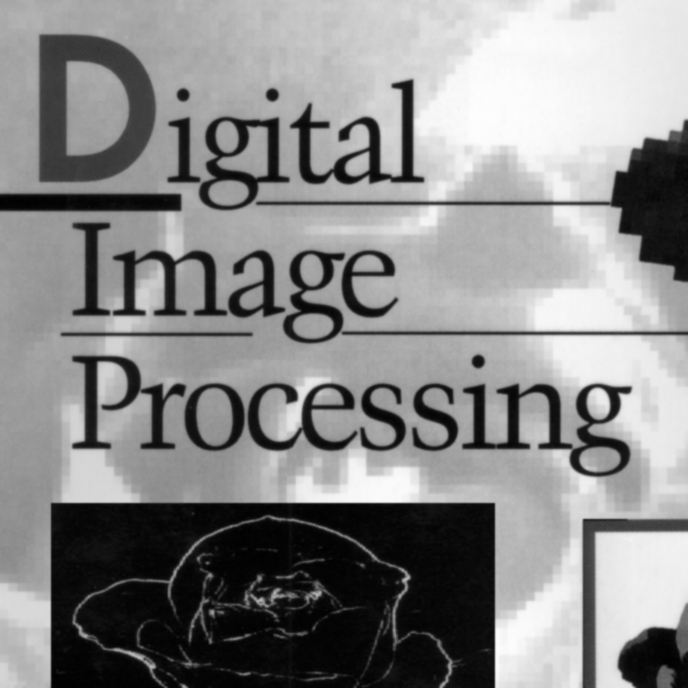
\includegraphics[width=\linewidth]{./images/5/original.jpg}}
        \caption{\small{Original image}}
    \end{minipage}
    \begin{minipage}{0.45\textwidth}
        \frame{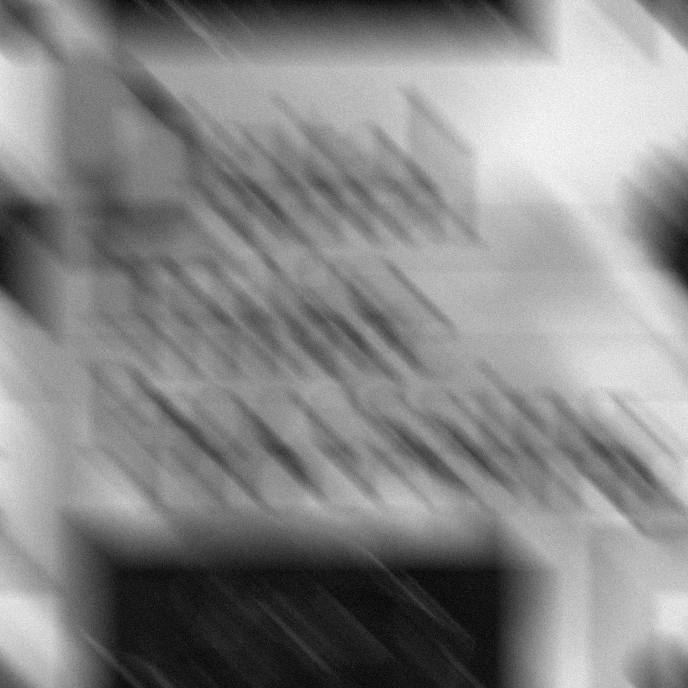
\includegraphics[width=\linewidth]{./images/5/blurred_noise_30.jpg}}
        \caption{\small{Blur + noise}}
    \end{minipage}
\end{figure}

\begin{figure}[!htb]\centering
    \begin{minipage}{0.45\textwidth}
        \frame{
\includegraphics[width=\linewidth]{./images/5/inv_blurred_noise_30.jpg}}
        \caption{\small{Inverse 'blur + noise'}}
    \end{minipage}
    \begin{minipage}{0.45\textwidth}
    \frame{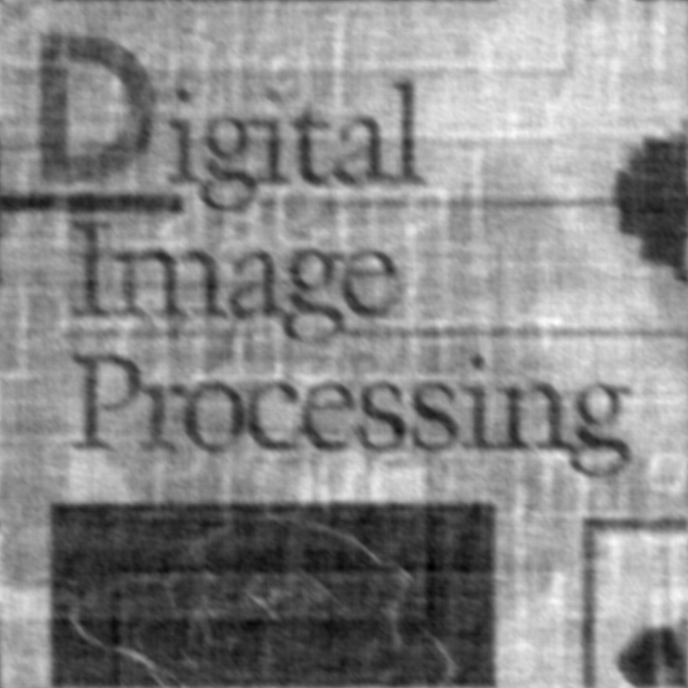
\includegraphics[width=\linewidth]{./images/5/wiener_blurred_noise_30.jpg}}
    \caption{\small{Wiener 'blur + noise'}}
    \end{minipage}
\end{figure}


\pagebreak
\subsubsection{Wiener performance}

\begin{figure}[!htb]\centering
    \begin{minipage}{0.45\textwidth}
        \frame{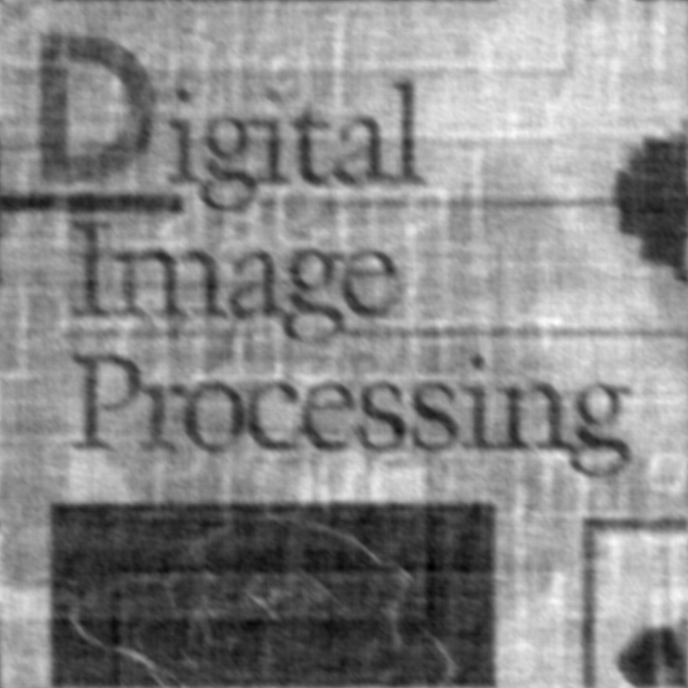
\includegraphics[width=\linewidth]{./images/5/wiener_blurred_noise_30.jpg}}
        \caption{\small{Wiener 'blur + noise ($\sigma^2 = 30$)'}}
    \end{minipage}
    \begin{minipage}{0.45\textwidth}
        \frame{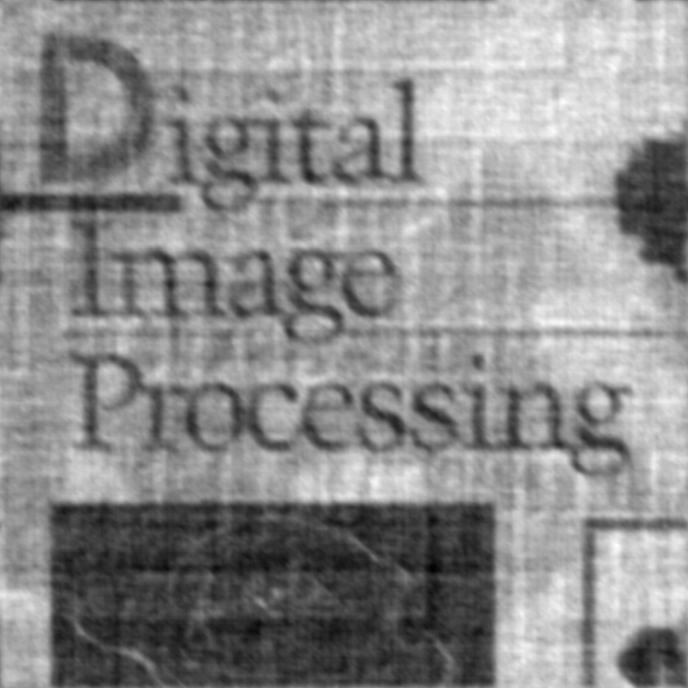
\includegraphics[width=\linewidth]{./images/5/wiener_blurred_noise_100.jpg}}
        \caption{\small{Wiener 'blur + noise ($\sigma^2 = 100$)'}}
    \end{minipage}
\end{figure}

\begin{figure}[!htb]\centering
    \begin{minipage}{0.45\textwidth}
        \frame{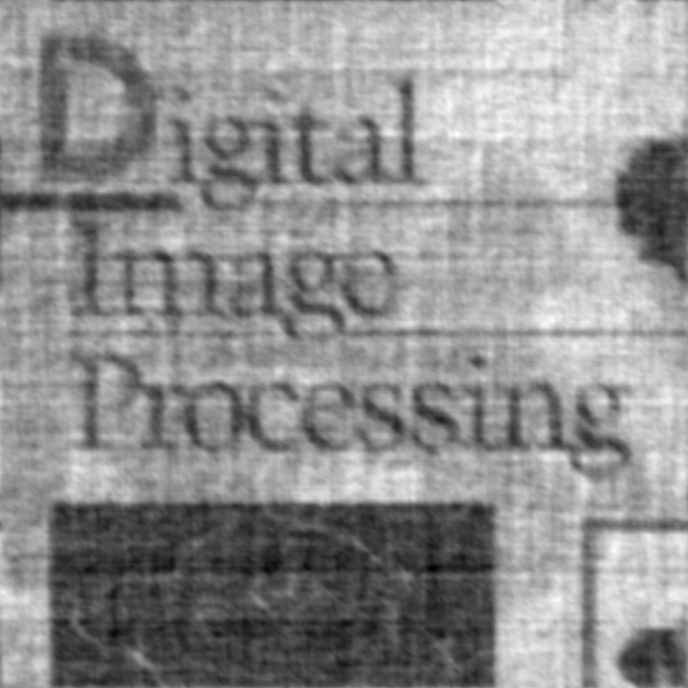
\includegraphics[width=\linewidth]{./images/5/wiener_blurred_noise_300.jpg}}
        \caption{\small{Inverse 'blur + noise ($\sigma^2 = 300$)'}}
    \end{minipage}
    \begin{minipage}{0.45\textwidth}
    \frame{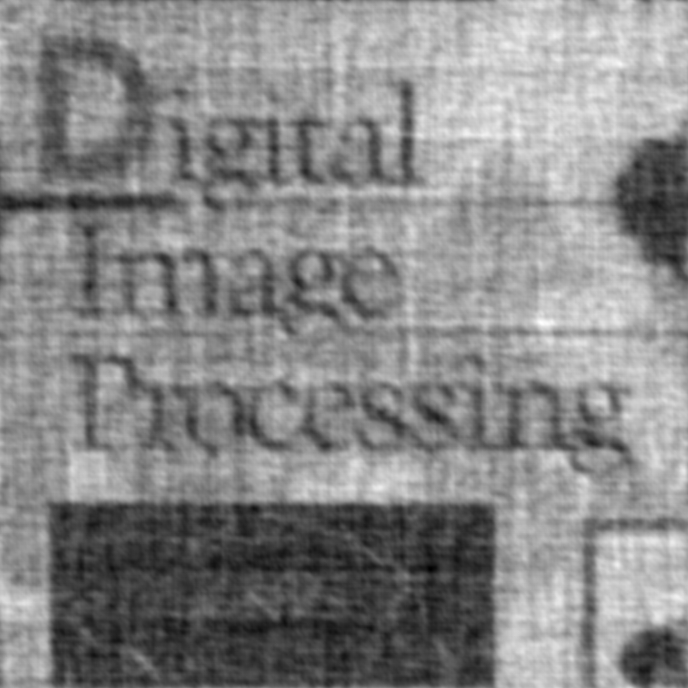
\includegraphics[width=\linewidth]{./images/5/wiener_blurred_noise.jpg}}
    \caption{\small{Wiener 'blur + noise ($\sigma^2 = 650$)'}}
    \end{minipage}
\end{figure}
